\documentclass[hyperref={pdfpagelabels=false}]{beamer}
\let\Tiny=\tiny

\usepackage{xspace}
\usepackage{xmpmulti}
\usepackage{array}
\usepackage[absolute,overlay]{textpos}
\usepackage{forloop}
\usepackage{comment}
\usecolortheme{rose}

\setbeamerfont{frametitle}{series=\bfseries}
\setbeamercolor*{title}{fg=white}
\setbeamercolor*{author}{fg=white}
\setbeamercolor*{institute}{fg=white}
\setbeamercolor*{date}{fg=white}
\setbeamerfont{title}{series=\bfseries,size=\huge}
% \setbeamercolor{frametitle}{}
\setbeamerfont{author}{series=\bfseries}

\useinnertheme{default}
\setbeamertemplate{navigation symbols}{}

\title{Adaptive Hierarchical Deep Reinforcement Learning}
\author{Florian Frei}
\institute{ETH Zurich -- Distributed Computing Group -- www.disco.ethz.ch}

\begin{document}

{
\usebackgroundtemplate{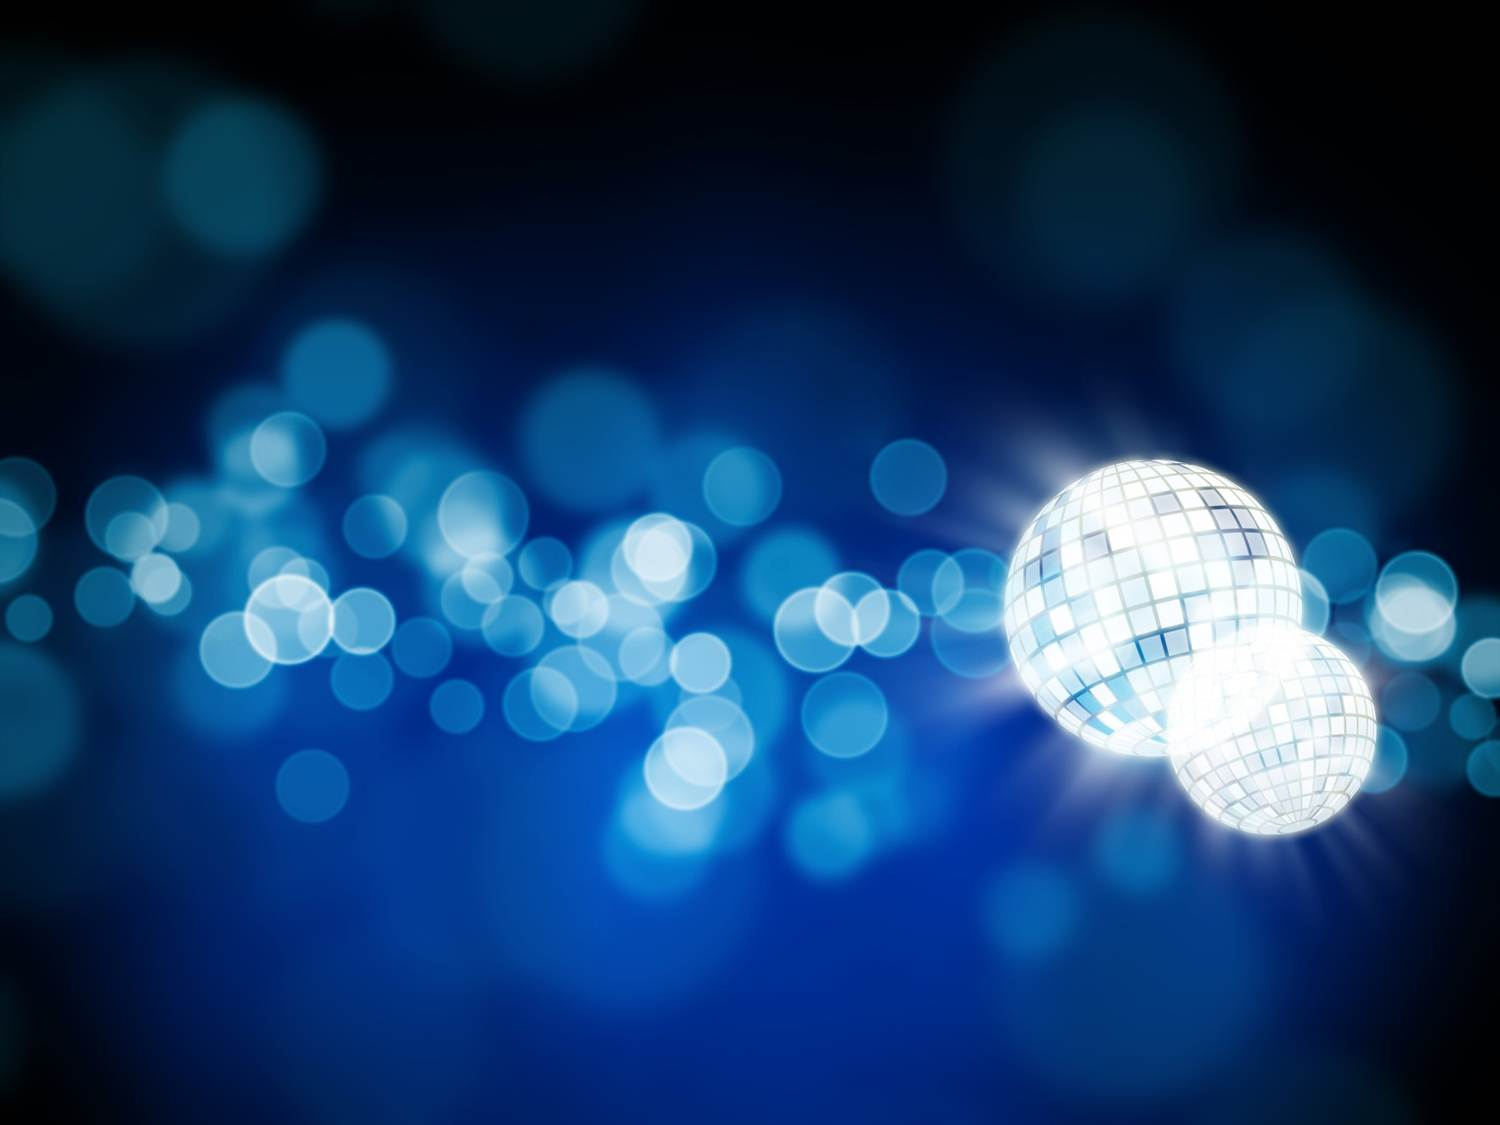
\includegraphics[width=\paperwidth]{figures/bg}}
\begin{frame}
	\begin{textblock*}{\paperwidth}[0,0](0cm,1cm)
		\begin{center}
			\usebeamercolor[fg]{title}
			\textbf{\huge \inserttitle}
		\end{center}
		\usebeamercolor[fg]{normal text}
	\end{textblock*}
	\begin{textblock*}{\paperwidth}[0,0](-0.5cm,7.4cm)
		\flushright
		\color{white}
		\itshape \insertauthor
		\usebeamercolor[fg]{normal text}
	\end{textblock*}
	\begin{textblock*}{\paperwidth}[0,1](0.2cm,9.4cm)
		\flushleft
 		\usebeamercolor[fg]{institute}
		\tiny \itshape \insertinstitute
		\usebeamercolor[fg]{normal text}
	\end{textblock*}
\end{frame}
}


\begin{frame}{Option-Critic Architecture}
\includegraphics[scale=0.6]{option_critic.pdf}
\end{frame}

\begin{frame}{Option-Critic Architecture}
\includegraphics[scale=0.7]{nn_schematic.pdf}
\end{frame}

\begin{frame}{Update Method}
\begin{gather*}
g_t = r_{t+1} + \gamma r_{t+2} + \ldots + \gamma^{T-1} r_{T}\\
Q(s_t , a_t) \leftarrow Q(s_t , a_t) + \alpha_t(g_t - Q(s_t , a_t))\\
Q(s_t , a_t) \leftarrow Q(s_t , a_t) + \alpha_t(q^{(n)}_t - Q(s_t , a_t)) \\
q^{(n)}_t  = r_{t+1} + \gamma r_{t+2} + \ldots + \gamma^{n-1} r_{t+n} + \gamma^n Q(s_{t+n}) , \;
\end{gather*}
\end{frame}


\begin{frame}{First experimental setting}
\includegraphics[scale=0.52]{first_exp.pdf}
\end{frame}

\begin{frame}{5-step method, no time pressure}
\includegraphics[scale=0.4]{./figures/local/4e_avrg_score_nt2.pdf}
\end{frame}

\begin{frame}{5-step method, no time pressure}
\includegraphics[scale=0.4]{./figures/local/3e_1x_avrg_score_nt2.pdf}
\end{frame}

\begin{frame}{5-step method, no time pressure}
\includegraphics[scale=0.4]{./figures/local/sl_ntime_0r.pdf}
\end{frame}

\begin{frame}{5-step method, time pressure}
\includegraphics[scale=0.4]{./figures/local/4e_avrg_score_t2.pdf}
\end{frame}

\begin{frame}{5-step method, time pressure}
\includegraphics[scale=0.4]{./figures/local/3e_1x_avrg_score_t2.pdf}
\end{frame}

\begin{frame}{5-step method, time pressure}
\includegraphics[scale=0.4]{./figures/local/sl_timepressure_sumary.pdf}
\end{frame}

\begin{frame}{MC method, no time pressure}
\includegraphics[scale=0.4]{./figures/mc/mc_ntime_wallterm_0.pdf}
\end{frame}

\begin{frame}{MC method, no time pressure}
\includegraphics[scale=0.4]{./figures/mc/mc_ntime_wallterm_-1.pdf}
\end{frame}

\begin{frame}{MC method, time pressure}
\includegraphics[scale=0.4]{./figures/mc/mc_time_wallterm_-0_1.pdf}
\end{frame}

\begin{frame}{MC method, $8\times8$ world}
\includegraphics[scale=0.4]{./figures/mc/8x8_score.pdf}
\end{frame}

\begin{frame}{Second experimental setting}
\includegraphics[scale=0.52]{second_exp.pdf}
\end{frame}

\begin{frame}{5-step method, no time pressure}
\includegraphics[scale=0.4]{./figures/local/local_score_key_nt_bade.pdf}
\end{frame}

\begin{frame}{5-step method, no time pressure}
\includegraphics[scale=0.4]{./figures/local/usage_key_nt_bade_run1.pdf}
\end{frame}

\begin{frame}{5-step method, no time pressure}
\includegraphics[scale=0.4]{./figures/local/local_score_key_nt_jump.pdf}
\end{frame}

\begin{frame}{5-step method, no time pressure}
\includegraphics[scale=0.4]{./figures/local/usage_key_nt_jump_run1.pdf}
\end{frame}

\begin{frame}{5-step method, time pressure}
\includegraphics[scale=0.4]{./figures/local/local_score_key_timep_bade.pdf}
\end{frame}

\begin{frame}{5-step method, time pressure}
\includegraphics[scale=0.4]{./figures/local/usage_key_timep_bade_run2.pdf}
\end{frame}

\begin{frame}{5-step method, time pressure}
\includegraphics[scale=0.4]{./figures/local/local_score_key_timep_jump.pdf}
\end{frame}

\begin{frame}{5-step method, time pressure}
\includegraphics[scale=0.4]{./figures/local/usage_key_timep_jump_run1.pdf}
\end{frame}

\begin{frame}{MC method, no time pressure}
\includegraphics[scale=0.4]{./figures/mc/score_key_0r_jumpe.pdf}
\end{frame}

\begin{frame}{MC method, no time pressure}
\includegraphics[scale=0.4]{./figures/mc/usage_0r_jumpe.pdf}
\end{frame}

\begin{frame}{MC method, no time pressure}
\includegraphics[scale=0.4]{./figures/mc/score_key_0r_bade.pdf}
\end{frame}

\begin{frame}{MC method, no time pressure}
\includegraphics[scale=0.4]{./figures/mc/usage_0r_bade.pdf}
\end{frame}

\begin{frame}{MC method, time pressure}
\includegraphics[scale=0.4]{./figures/mc/score_key_0r_timep_jumpe.pdf}
\end{frame}

\begin{frame}{MC method, time pressure}
\includegraphics[scale=0.4]{./figures/mc/usage_0r_timep_jumpe_run1.pdf}
\end{frame}

\begin{frame}{MC method, time pressure}
\includegraphics[scale=0.4]{./figures/mc/score_key_0r_timep_bade.pdf}
\end{frame}

\begin{frame}{MC method, time pressure}
\includegraphics[scale=0.4]{./figures/mc/usage_0r_timep_bade_run2.pdf}
\end{frame}

\begin{comment}

\includegraphics[scale=0.25]{./figures/mc/usage_0r_timep_jumpe_run5.pdf}
\includegraphics[scale=0.25]{./figures/mc/usage_0r_timep_jumpe_run4.pdf}

\end{comment}

\begin{frame}{QnA}

\end{frame}



\end{document}